%iffalse
\let\negmedspace\undefined
\let\negthickspace\undefined
\documentclass[journal,12pt,onecolumn]{IEEEtran}
\usepackage{cite}
\usepackage{amsmath,amssymb,amsfonts,amsthm}
\usepackage{algorithmic}
\usepackage{graphicx}
\usepackage{textcomp}
\usepackage{xcolor}
\usepackage{txfonts}
\usepackage{listings}
\usepackage{enumitem}
\usepackage{mathtools}
\usepackage{newunicodechar}
\newunicodechar{₹}{\text{Rs.}}
\usepackage{gensymb}
\usepackage{comment}
\usepackage[breaklinks=true]{hyperref}
\usepackage{tkz-euclide} 
\usepackage{listings}
\usepackage{gvv}
\def\inputGnumericTable{}                                 
\usepackage[utf8]{inputenc}                              
\usepackage{color}                                         
\usepackage{array}                                        
\usepackage{longtable}                                     
\usepackage{calc}                                          
\usepackage{multirow}                                      
\usepackage{hhline}                                        
\usepackage{ifthen}                                        
\usepackage{lscape}
\newtheorem{theorem}{Theorem}[section]
\newtheorem{problem}{Problem}
\newtheorem{proposition}{Proposition}[section]
\newtheorem{lemma}{Lemma}[section]
\newtheorem{corollary}[theorem]{Corollary}
\newtheorem{example}{Example}[section]
\newtheorem{definition}[problem]{Definition}
\newcommand{\BEQA}{\begin{eqnarray}}
\newcommand{\EEQA}{\end{eqnarray}}
\newcommand{\define}{\stackrel{\triangle}{=}}
\theoremstyle{remark}
\newtheorem{rem}{Remark}
\graphicspath{ {./Figures/} }
\usepackage{float} % For the [H] float option
\usepackage{textcomp}
\usepackage{multicol}

\begin{document}
\begin{enumerate}[start=1, label=Q.\arabic*]

\item The ratio of boys to girls in a class is $7$ to $3$.  
Among the options below, an acceptable value for the total number of students in the class is:
\begin{enumerate}
\begin{multicols}{4}
\item 21
\item 37
\item 50
\item 73
\end{multicols}
\end{enumerate}

\hfill{\brak{\text{GATE MA 2021}}}


\item A polygon is convex if, for every pair of points $P$ and $Q$ belonging to the polygon, the line segment $PQ$ lies completely inside or on the polygon.  
Which one of the following is NOT a convex polygon?
\begin{enumerate}
\item \begin{figure}[H]
\includegraphics[width=0.15\columnwidth]{Figures/qt2a.png}\caption*{}\end{figure}
\item \begin{figure}[H]
\includegraphics[width=0.15\columnwidth]{Figures/qn2b.png}\caption*{}\end{figure}
\item \begin{figure}[H]
\includegraphics[width=0.15\columnwidth]{Figures/qn2c.png}\caption*{}\end{figure}
\item \begin{figure}[H]
\includegraphics[width=0.15\columnwidth]{Figures/qn2d.png}\caption*{}\end{figure}
\end{enumerate}

\hfill{\brak{\text{GATE MA 2021}}}


\item Consider the following sentences:  

(i) Everybody in the class is prepared for the exam.  
(ii) Babu invited Danish to his home because he enjoys playing chess.  

Which of the following is the CORRECT observation about the above two sentences?
\begin{enumerate}
\begin{multicols}{2}
\item (i) is grammatically correct and (ii) is unambiguous
\item (i) is grammatically incorrect and (ii) is unambiguous
\item (i) is grammatically correct and (ii) is ambiguous
\item (i) is grammatically incorrect and (ii) is ambiguous
\end{multicols}
\end{enumerate}

\hfill{\brak{\text{GATE MA 2021}}}


\item A circular sheet of paper is folded along the lines in the directions shown.  
The paper, after being punched in the final folded state as shown and unfolded in the reverse order of folding, will look like:
\begin{figure}
    \centering
    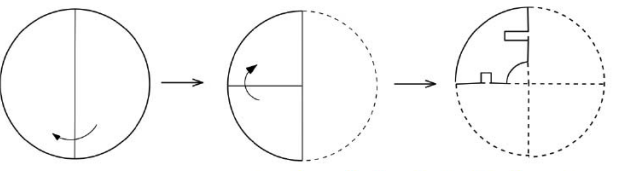
\includegraphics[width=0.5\columnwidth]{Figures/qn4.png}
    \caption{Caption}
\end{figure}
\begin{enumerate}
\item \begin{figure}[H]
\includegraphics[width=0.25\columnwidth]{Figures/qn4a.png}\caption*{}\end{figure}
\item \begin{figure}[H]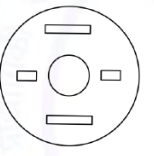
\includegraphics[width=0.25\columnwidth]{Figures/qn4b.png}\caption*{}\end{figure}
\item \begin{figure}[H]
\includegraphics[width=0.25\columnwidth]{Figures/qn4c.png}\caption*{}\end{figure}
\item \begin{figure}[H]
\includegraphics[width=0.25\columnwidth]{Figures/qn4d.png}\caption*{}\end{figure}
\end{enumerate}

\hfill{\brak{\text{GATE MA 2021}}}


\item \brak{\text{Surgery is to surgeon as writer is to \underline{\hspace{2cm}}}}  

Which one of the following options maintains a similar logical relation in the above sentence?
\begin{enumerate}
\begin{multicols}{2}
\item Plan, outline
\item Hospital, library
\item Doctor, book
\item Medicine, grammar
\end{multicols}
\end{enumerate}

\hfill{\brak{\text{GATE MA 2021}}}

\item We have two rectangular sheets of paper, $M$ and $N$, of dimensions $6 \,\text{cm} \times 1 \,\text{cm}$ each.  
Sheet $M$ is rolled to form an open cylinder by bringing the short edges of the sheet together.  
Sheet $N$ is cut into equal square patches and assembled to form the largest possible closed cube.  
Assuming the ends of the cylinder are closed, the ratio of the volume of the cylinder to that of the cube is
\begin{enumerate}
\begin{multicols}{4}
\item $\dfrac{2}{\pi}$
\item $\dfrac{3}{\pi}$
\item $2\pi$
\item $3\pi$
\end{multicols}
\end{enumerate}

\hfill{\brak{\text{GATE MA 2021}}}
\item 


\noindent Details of prices of two items P and Q are presented in the above table.  
The ratio of cost of item P to cost of item Q is $3: 4$.  
Discount is calculated as the difference between the marked price and the selling price.  
The profit percentage is calculated as the ratio of the difference between selling price and cost, to the cost \brak{\text{Profit \% } = \dfrac{\text{Selling price} - \text{Cost}}{\text{Cost}} \times 100}.  

The discount on item Q, as a percentage of its marked price, is \underline{\hspace{2cm}}.
\begin{table}[H]
\centering
\caption*{}
\label{tab:pricesPQ}
\begin{tabular}{|c|c|c|c|}
\hline
\text{Items} & \text{Cost \brak{\text{₹}}} & \text{Profit \%} & \text{Marked Price \brak{\text{₹}}} \\ \hline
\text{P} & 5{,}400 & \text{---} & 5{,}860 \\ \hline
\text{Q} & \text{---} & 25 & 10{,}000 \\ \hline
\end{tabular}
\end{table}
\begin{enumerate}
\item 25
\item 12.5
\item 10
\item 5
\end{enumerate}

\hfill{\brak{\text{GATE MA 2021}}}


\item There are five bags each containing identical sets of ten distinct chocolates.  
One chocolate is picked from each bag. The probability that at least two chocolates are identical is \underline{\hspace{2cm}}.
\begin{enumerate}
\item 0.3024
\item 0.4235
\item 0.6976
\item 0.8125
\end{enumerate}

\hfill{\brak{\text{GATE MA 2021}}}
\item Given below are two statements 1 and 2, and two conclusions I and II.  

Statement 1: All bacteria are microorganisms.  
Statement 2: All pathogens are microorganisms.  

Conclusion I: Some pathogens are bacteria.  
Conclusion II: All pathogens are not bacteria.  

Based on the above statements and conclusions, which one of the following options is logically CORRECT?
\begin{enumerate}
\item Only conclusion I is correct
\item Only conclusion II is correct
\item Either conclusion I or II is correct
\item Neither conclusion I nor II is correct
\end{enumerate}

\hfill{\brak{\text{GATE MA 2021}}}


\item Some people suggest anti-obesity measures \brak{\text{AOM}} such as displaying calorie information in restaurant menus.  
Such measures sidestep addressing the core problems that cause obesity\brak{:} poverty and income inequality.  
Which one of the following statements summarizes the passage?
\begin{enumerate}
\item The proposed AOM addresses the core problems that cause obesity
\item If obesity reduces, poverty will naturally reduce, since obesity causes poverty
\item AOM are addressing the core problems and are likely to succeed
\item AOM are addressing the problem superficially
\end{enumerate}

\hfill{\brak{\text{GATE MA 2021}}}
\item Let $A$ be a $3 \times 4$ matrix and $B$ be a $4 \times 3$ matrix with real entries such that $AB$ is non\mbox{-}singular. Consider the following statements\brak{:}

P : Nullity of $A$ is $0$.\\
Q : $BA$ is a non\mbox{-}singular matrix.\\

Then
\begin{enumerate}
\item both P and Q are TRUE
\item P is TRUE and Q is FALSE
\item P is FALSE and Q is TRUE
\item both P and Q are FALSE
\end{enumerate}

\hfill{\brak{\text{GATE MA 2021}}}
\item Let $f(z)=u(x,y)+i v(x,y)$ for $z=x+iy \in \mathbb{C}$, where $x$ and $y$ are real numbers, be a non\mbox{-}constant analytic function on the complex plane $\mathbb{C}$.  
Let $u_x, v_x$ and $u_y, v_y$ denote the first order partial derivatives of $u(x,y)=\Re(f(z))$ and $v(x,y)=\Im(f(z))$ with respect to real variables $x$ and $y$, respectively.  

Consider the following two functions defined on $\mathbb{C}$:  
\[
g_1(z)=u_x(x,y)-i u_y(x,y), \quad g_2(z)=v_x(x,y)+i v_y(x,y), \quad \text{for } z=x+iy \in \mathbb{C}.
\]

Then
\begin{enumerate}
\item both $g_1(z)$ and $g_2(z)$ are analytic in $\mathbb{C}$
\item $g_1(z)$ is analytic in $\mathbb{C}$ and $g_2(z)$ is NOT analytic in $\mathbb{C}$
\item $g_1(z)$ is NOT analytic in $\mathbb{C}$ and $g_2(z)$ is analytic in $\mathbb{C}$
\item neither $g_1(z)$ nor $g_2(z)$ is analytic in $\mathbb{C}$
\end{enumerate}

\hfill{\brak{\text{GATE MA 2021}}}


\item Let $T(z)=\dfrac{az+b}{cz+d},\ ad-bc \ne 0$, be the Möbius transformation which maps the points $z_1=0,\ z_2=-i,\ z_3=\infty$ in the $z$\mbox{-}plane onto the points $w_1=10,\ w_2=5-5i,\ w_3=5+5i$ in the $w$\mbox{-}plane, respectively.  

Then the image of the set $S=\{z \in \mathbb{C} : \Re(z)<0\}$ under the map $w=T(z)$ is
\begin{enumerate}
\item $\{w \in \mathbb{C} : \abs{w}<5\}$
\item $\{w \in \mathbb{C} : \abs{w}>5\}$
\item $\{w \in \mathbb{C} : \abs{w-5}<5\}$
\item $\{w \in \mathbb{C} : \abs{w-5}>5\}$
\end{enumerate}

\hfill{\brak{\text{GATE MA 2021}}}
\item Let $R$ be the row reduced echelon form of a $4 \times 4$ real matrix $A$ and let the third column of $R$ be 
\[
\myvec{0 \\ 1 \\ 0 \\ 0}.
\]  

Consider the following statements\brak{:}

P : If $\myvec{\alpha \\ \beta \\ \gamma \\ 0}$ is a solution of $Ax=0$, then $\gamma=0$.\\
Q : For all $b \in \mathbb{R}^{4},\ \text{rank}[A|b]=\text{rank}[R|b]$.\\

Then
\begin{enumerate}
\item both P and Q are TRUE
\item P is TRUE and Q is FALSE
\item P is FALSE and Q is TRUE
\item both P and Q are FALSE
\end{enumerate}

\hfill{\brak{\text{GATE MA 2021}}}


\item The eigenvalues of the boundary value problem
\[
\dfrac{d^{2}y}{dx^{2}}+\lambda y=0,\quad x \in \brak{0,\pi},\;\; \lambda>0,
\]
\[
y\brak{0}=0,\quad y\brak{\pi}-\dfrac{dy}{dx}\brak{\pi}=0,
\]
are given by
\begin{enumerate}
\item $\lambda=\brak{n\pi}^{2},\quad n=1,2,3,\dots$
\item $\lambda=n^{2},\quad n=1,2,3,\dots$
\item $\lambda=k_{n}^{2},\quad \text{where } k_{n}, n=1,2,3,\dots \text{ are the roots of } k-\tan\brak{k\pi}=0$
\item $\lambda=k_{n}^{2},\quad \text{where } k_{n}, n=1,2,3,\dots \text{ are the roots of } k+\tan\brak{k\pi}=0$
\end{enumerate}

\hfill{\brak{\text{GATE MA 2021}}}
\item The family of surfaces given by $u=xy+f\brak{x^{2}-y^{2}}$, where $f : \mathbb{R}\to\mathbb{R}$ is a differentiable function, satisfies
\begin{enumerate}
\item $x\dfrac{\partial u}{\partial x}+x\dfrac{\partial u}{\partial y}=x^{2}+y^{2}$
\item $x\dfrac{\partial u}{\partial x}+y\dfrac{\partial u}{\partial y}=x^{2}+y^{2}$
\item $x\dfrac{\partial u}{\partial x}+x\dfrac{\partial u}{\partial y}=x^{2}-y^{2}$
\item $x\dfrac{\partial u}{\partial x}+y\dfrac{\partial u}{\partial y}=x^{2}-y^{2}$
\end{enumerate}

\hfill{\brak{\text{GATE MA 2021}}}


\item The function $u(x,t)$ satisfies the initial value problem
\[
\dfrac{\partial^{2}u}{\partial t^{2}}=\dfrac{\partial^{2}u}{\partial x^{2}},\quad x \in \mathbb{R},\; t>0,
\]
\[
u(x,0)=0,\quad \dfrac{\partial u}{\partial t}\brak{x,0}=4x e^{-x^{2}}.
\]
Then $u(5,5)$ is
\begin{enumerate}
\item $1-\dfrac{1}{e^{100}}$
\item $1-e^{100}$
\item $1-\dfrac{1}{e^{10}}$
\item $1-e^{10}$
\end{enumerate}

\hfill{\brak{\text{GATE MA 2021}}}
\item Consider the fixed\mbox{-}point iteration
\[
x_{n+1}=\varphi\brak{x_{n}},\quad n \ge 0,
\]
with
\[
\varphi(x)=3+(x-3)^{3},\quad x \in \brak{2.5,3.5},
\]
and the initial approximation $x_{0}=3.25$.  

Then, the order of convergence of the fixed\mbox{-}point iteration method is
\begin{enumerate}
\begin{multicols}{4}
\item 1
\item 2
\item 3
\item 4
\end{multicols}
\end{enumerate}

\hfill{\brak{\text{GATE MA 2021}}}


\item Let $\{e_{n} : n=1,2,3,\dots\}$ be an orthonormal basis of a complex Hilbert space $H$.  
Consider the following statements\brak{:}

P : There exists a bounded linear functional $f : H \to \mathbb{C}$ such that $f(e_{n})=\tfrac{1}{n}$ for $n=1,2,3,\dots$  

Q : There exists a bounded linear functional $g : H \to \mathbb{C}$ such that $g(e_{n})=\tfrac{1}{\sqrt{n}}$ for $n=1,2,3,\dots$  

Then
\begin{enumerate}
\item both P and Q are TRUE
\item P is TRUE and Q is FALSE
\item P is FALSE and Q is TRUE
\item both P and Q are FALSE
\end{enumerate}

\hfill{\brak{\text{GATE MA 2021}}}

\item Let $f : \brak{-\tfrac{\pi}{2},\tfrac{\pi}{2}} \to \mathbb{R}$ be given by $f(x)=\tfrac{\pi}{2}+x-\tan^{-1}x$.  
Consider the following statements\brak{:}

P : $\abs{f(x)-f(y)}<\abs{x-y}$ for all $x,y \in \brak{-\tfrac{\pi}{2},\tfrac{\pi}{2}}$.\\
Q : $f$ has a fixed point.\\

Then
\begin{enumerate}
\item both P and Q are TRUE
\item P is TRUE and Q is FALSE
\item P is FALSE and Q is TRUE
\item both P and Q are FALSE
\end{enumerate}

\hfill{\brak{\text{GATE MA 2021}}}


\item Consider the following statements\brak{:}

P : $d_{1}(x,y)=\abs{\log\brak{\tfrac{x}{y}}}$ is a metric on $\brak{0,1}$.\\
Q : $d_{2}(x,y)=
\begin{cases}
\abs{x}+\abs{y}, & \text{if } x \ne y,\\
0, & \text{if } x=y,
\end{cases}
\ \ \text{is a metric on } \brak{0,1}.
$

Then
\begin{enumerate}
\item both P and Q are TRUE
\item P is TRUE and Q is FALSE
\item P is FALSE and Q is TRUE
\item both P and Q are FALSE
\end{enumerate}

\hfill{\brak{\text{GATE MA 2021}}}
\item Let $f : \mathbb{R}^{3}\to \mathbb{R}$ be a twice continuously differentiable scalar field such that $\text{div}\brak{\nabla f}=6$.  
Let $S$ be the surface $x^{2}+y^{2}+z^{2}=1$ and $\hat{n}$ be unit outward normal to $S$.  
Then the value of 
\[
\iint_{S}\brak{\nabla f \cdot \hat{n}}\, dS
\] 
is
\begin{enumerate}
\begin{multicols}{4}
\item $2\pi$
\item $4\pi$
\item $6\pi$
\item $8\pi$
\end{multicols}
\end{enumerate}

\hfill{\brak{\text{GATE MA 2021}}}


\item Consider the following statements\brak{:}

P : Every compact metrizable topological space is separable.\\
Q : Every Hausdorff topology on a finite set is metrizable.\\

Then
\begin{enumerate}
\item both P and Q are TRUE
\item P is TRUE and Q is FALSE
\item P is FALSE and Q is TRUE
\item both P and Q are FALSE
\end{enumerate}

\hfill{\brak{\text{GATE MA 2021}}}


\item Consider the following topologies on the set $\mathbb{R}$ of all real numbers\brak{:}

$T_{1}=\{U \subset \mathbb{R} : 0 \notin U \text{ or } U=\mathbb{R}\},$  

$T_{2}=\{U \subset \mathbb{R} : 0 \in U \text{ or } U=\varnothing\},$  

$T_{3}=T_{1} \cap T_{2}$.  

Then the closure of the set $\{1\}$ in $\brak{\mathbb{R},T_{3}}$ is
\begin{enumerate}
\begin{multicols}{4}
\item $\{1\}$
\item $\{0,1\}$
\item $\mathbb{R}$
\item $\mathbb{R}\setminus\{0\}$
\end{multicols}
\end{enumerate}

\hfill{\brak{\text{GATE MA 2021}}}
\item Let $f : \mathbb{R}^{2}\to \mathbb{R}$ be differentiable.  
Let $D_{u}f\brak{0,0}$ and $D_{v}f\brak{0,0}$ be the directional derivatives of $f$ at $\brak{0,0}$ in the directions of the unit vectors 
$u=\brak{\tfrac{1}{\sqrt{5}},\tfrac{2}{\sqrt{5}}}$ and $v=\brak{\tfrac{1}{\sqrt{2}},\tfrac{-1}{\sqrt{2}}}$, respectively.  
If $D_{u}f\brak{0,0}=\sqrt{5}$ and $D_{v}f\brak{0,0}=\sqrt{2}$, then $\tfrac{\partial f}{\partial x}\brak{0,0}+\tfrac{\partial f}{\partial y}\brak{0,0}=$ \underline{\hspace{2cm}}.

\hfill{\brak{\text{GATE MA 2021}}}


\item Let $\Gamma$ denote the boundary of the square region $R$ with vertices $\brak{0,0},\ \brak{2,0},\ \brak{2,2}$ and $\brak{0,2}$ oriented in the counter\mbox{-}clockwise direction.  
Then
\[
\oint_{\Gamma}\brak{1-y^{2}}\,dx+x\,dy=\underline{\hspace{2cm}}.
\]

\hfill{\brak{\text{GATE MA 2021}}}


\item The number of $5$\mbox{-}Sylow subgroups in the symmetric group $S_{5}$ of degree $5$ is \underline{\hspace{2cm}}.

\hfill{\brak{\text{GATE MA 2021}}}


\item Let $I$ be the ideal generated by $x^{2}+x+1$ in the polynomial ring $R=\mathbb{Z}_{3}[x]$, where $\mathbb{Z}_{3}$ denotes the ring of integers modulo $3$.  
Then the number of units in the quotient ring $R/I$ is \underline{\hspace{2cm}}.

\hfill{\brak{\text{GATE MA 2021}}}


\item Let $T : \mathbb{R}^{3}\to \mathbb{R}^{3}$ be a linear transformation such that
\[
T\!\left(\myvec{1\\1\\1}\right)=\myvec{1\\-1\\1},\quad 
T^{2}\!\left(\myvec{1\\1\\1}\right)=\myvec{1\\1\\1},\quad 
T^{2}\!\left(\myvec{1\\2\\1}\right)=\myvec{1\\1\\1}.
\]
Then the rank of $T$ is \underline{\hspace{2cm}}.

\hfill{\brak{\text{GATE MA 2021}}}
\item Let $y(x)$ be the solution of the following initial value problem
\[
x^{2}\dfrac{d^{2}y}{dx^{2}}-4x\dfrac{dy}{dx}+6y=0,\quad x>0,
\]
\[
y(2)=0,\quad \dfrac{dy}{dx}\brak{2}=4.
\]
Then $y(4)=$ \underline{\hspace{2cm}}.

\hfill{\brak{\text{GATE MA 2021}}}


\item Let 
\[
f(x)=x^{4}+2x^{3}-11x^{2}-12x+36,\quad x \in \mathbb{R}.
\]
The order of convergence of the Newton–Raphson method
\[
x_{n+1}=x_{n}-\dfrac{f(x_{n})}{f^{\prime}(x_{n})},\quad n \ge 0,
\]
with $x_{0}=2.1$, for finding the root $\alpha=2$ of the equation $f(x)=0$ is \underline{\hspace{2cm}}.

\hfill{\brak{\text{GATE MA 2021}}}


\item If the polynomial
\[
p(x)=\alpha+\beta(x+2)+\gamma(x+2)(x+1)+\delta(x+2)(x+1)x
\]
interpolates the data
\begin{table}[H]
\centering
\caption*{}
\label{tab:interp}
\begin{tabular}{|c|c|c|c|c|c|}
\hline
$x$ & $-2$ & $-1$ & $0$ & $1$ & $2$ \\ \hline
$f(x)$ & $2$ & $-1$ & $8$ & $5$ & $-34$ \\ \hline
\end{tabular}
\end{table}

then $\alpha+\beta+\gamma+\delta=$ \underline{\hspace{2cm}}.

\hfill{\brak{\text{GATE MA 2021}}}
\item Consider the Linear Programming Problem $P$\brak{:}  
Maximize $2x_{1}+3x_{2}$  
subject to
\[
2x_{1}+x_{2}\leq 6,\quad -x_{1}+x_{2}\leq 1,\quad x_{1}+x_{2}\leq 3,\quad x_{1}\geq 0,\ x_{2}\geq 0.
\]  
Then the optimal value of the dual of $P$ is equal to \underline{\hspace{2cm}}.

\hfill{\brak{\text{GATE MA 2021}}}


\item Consider the Linear Programming Problem $P$\brak{:}  
Minimize $2x_{1}-5x_{2}$  
subject to
\[
2x_{1}+3x_{2}+s_{1}=12,\quad -x_{1}+x_{2}+s_{2}=1,\quad -x_{1}+2x_{2}+s_{3}=3,
\]
\[
x_{1}\geq 0,\ x_{2}\geq 0,\ s_{1}\geq 0,\ s_{2}\geq 0,\ s_{3}\geq 0.
\]  
If $\myvec{x_{1}\\x_{2}\\s_{1}\\s_{2}\\s_{3}}$ is a basic feasible solution of $P$, then $x_{1}+s_{1}+s_{2}+s_{3}=$ \underline{\hspace{2cm}}.

\hfill{\brak{\text{GATE MA 2021}}}


\item Let $H$ be a complex Hilbert space. Let $u,v \in H$ be such that $\brak{u,v}=2$. Then
\[
\dfrac{1}{2\pi}\int_{0}^{2\pi}\abs{u+e^{it}v}^{2}e^{it}\,dt=\underline{\hspace{2cm}}.
\]

\hfill{\brak{\text{GATE MA 2021}}}

\item Let $\mathbb{Z}$ denote the ring of integers. Consider the subring
\[
R=\{a+b\sqrt{-17}: a,b \in \mathbb{Z}\}
\]
of the field $\mathbb{C}$ of complex numbers.  

Consider the following statements\brak{:}

P : $2+\sqrt{-17}$ is an irreducible element.\\
Q : $2+\sqrt{-17}$ is a prime element.\\

Then
\begin{enumerate}
\item both P and Q are TRUE
\item P is TRUE and Q is FALSE
\item P is FALSE and Q is TRUE
\item both P and Q are FALSE
\end{enumerate}

\hfill{\brak{\text{GATE MA 2021}}}


\item Consider the second\mbox{-}order partial differential equation \brak{\text{PDE}}
\[
\dfrac{\partial^{2}u}{\partial x^{2}}+4\dfrac{\partial^{2}u}{\partial x \partial y}+\brak{x^{2}+4y^{2}}\dfrac{\partial^{2}u}{\partial y^{2}}=\sin\brak{x+y}.
\]

Consider the following statements\brak{:}

P : The PDE is parabolic on the ellipse $\dfrac{x^{2}}{4}+y^{2}=1$.\\
Q : The PDE is hyperbolic inside the ellipse $\dfrac{x^{2}}{4}+y^{2}=1$.\\

Then
\begin{enumerate}
\item both P and Q are TRUE
\item P is TRUE and Q is FALSE
\item P is FALSE and Q is TRUE
\item both P and Q are FALSE
\end{enumerate}

\hfill{\brak{\text{GATE MA 2021}}}
\item If $u(x,y)$ is the solution of the Cauchy problem
\[
x\dfrac{\partial u}{\partial x}+\dfrac{\partial u}{\partial y}=1,\quad u(x,0)=-x^{2},\; x>0,
\]
then $u(2,1)$ is equal to
\begin{enumerate}
\begin{multicols}{2}
\item $1-2e^{-2}$
\item $1+4e^{-2}$
\item $1-4e^{-2}$
\item $1+2e^{-2}$
\end{multicols}
\end{enumerate}

\hfill{\brak{\text{GATE MA 2021}}}


\item Let $y(t)$ be the solution of the initial value problem
\[
\dfrac{d^{2}y}{dt^{2}}+a\dfrac{dy}{dt}+by=f(t),\quad a>0,\ b>0,\ a\ne b,\ a^{2}-4b=0,
\]
\[
y(0)=0,\quad \dfrac{dy}{dt}(0)=0,
\]
obtained by the method of Laplace transform. Then
\begin{enumerate}
\item $y(t)=\int_{0}^{t}\tau e^{-\tfrac{a\tau}{2}}f(t-\tau)\,d\tau$
\item $y(t)=\int_{0}^{t}e^{-\tfrac{a\tau}{2}}f(t-\tau)\,d\tau$
\item $y(t)=\int_{0}^{t}\tau e^{-\tfrac{b\tau}{2}}f(t-\tau)\,d\tau$
\item $y(t)=\int_{0}^{t}e^{-\tfrac{b\tau}{2}}f(t-\tau)\,d\tau$
\end{enumerate}

\hfill{\brak{\text{GATE MA 2021}}}
\item The critical point of the differential equation
\[
\dfrac{d^{2}y}{dt^{2}}+2\alpha\dfrac{dy}{dt}+\beta^{2}y=0,\quad \alpha>\beta>0,
\]
is a
\begin{enumerate}
\item node and is asymptotically stable
\item spiral point and is asymptotically stable
\item node and is unstable
\item saddle point and is unstable
\end{enumerate}

\hfill{\brak{\text{GATE MA 2021}}}


\item The initial value problem
\[
\dfrac{dy}{dt}=f(t,y),\quad t>0,\quad y(0)=1,
\]
where $f(t,y)=-10y$, is solved by the following Euler method
\[
y_{n+1}=y_{n}+h f(t_{n},y_{n}),\quad n \ge 0,
\]
with step\mbox{-}size $h$. Then $y_{n}\to 0$ as $n \to \infty$, provided
\begin{enumerate}
\item $0<h<0.2$
\item $0.3<h<0.4$
\item $0.4<h<0.5$
\item $0.5<h<0.55$
\end{enumerate}

\hfill{\brak{\text{GATE MA 2021}}}
\item Consider the Linear Programming Problem $P$\brak{:}  
Maximize $c_{1}x_{1}+c_{2}x_{2}$  

subject to
\[
a_{11}x_{1}+a_{12}x_{2}\leq b_{1},\quad
a_{21}x_{1}+a_{22}x_{2}\leq b_{2},\quad
a_{31}x_{1}+a_{32}x_{2}\leq b_{3},
\]
\[
x_{1}\geq 0,\ x_{2}\geq 0,\ \text{where } a_{ij}, b_{i}, c_{j} \text{ are real numbers } \brak{i=1,2,3;\ j=1,2}.
\]

Let $\myvec{p\\q}$ be a feasible solution of $P$ such that $pc_{1}+qc_{2}=6$ and let all feasible solutions $\myvec{x_{1}\\x_{2}}$ of $P$ satisfy $-5\leq c_{1}x_{1}+c_{2}x_{2}\leq 12$.  

Then, which one of the following statements is NOT true?  
\begin{enumerate}
\item $P$ has an optimal solution
\item The feasible region of $P$ is a bounded set
\item If $\myvec{y_{1}\\y_{2}\\y_{3}}$ is a feasible solution of the dual of $P$, then $b_{1}y_{1}+b_{2}y_{2}+b_{3}y_{3}\geq 6$
\item The dual of $P$ has at least one feasible solution
\end{enumerate}

\hfill{\brak{\text{GATE MA 2021}}}


\item Let $L^{2}\brak{-1,1}$ be the Hilbert space of real valued square integrable functions on $\brak{-1,1}$ equipped with the norm 
\[
\lVert f \rVert=\left(\int_{-1}^{1}\abs{f(x)}^{2}\,dx\right)^{\tfrac{1}{2}}.
\]

Consider the subspace $M=\{f \in L^{2}\brak{-1,1} : \int_{-1}^{1}f(x)\,dx=0\}$.  

For $f(x)=x^{2}$, define $d=\inf\{\lVert f-g \rVert : g \in M\}$. Then
\begin{enumerate}
\begin{multicols}{2}
\item $d=\tfrac{\sqrt{2}}{3}$
\item $d=\tfrac{2}{3}$
\item $d=\tfrac{3}{\sqrt{2}}$
\item $d=\tfrac{3}{2}$
\end{multicols}
\end{enumerate}

\hfill{\brak{\text{GATE MA 2021}}}
\item Let $C[0,1]$ be the Banach space of real valued continuous functions on $\brak{0,1}$ equipped with the supremum norm.  
Define $T : C[0,1]\to C[0,1]$ by
\[
(Tf)(x)=\int_{0}^{x}t f(t)\,dt.
\]

Let $R(T)$ denote the range space of $T$. Consider the following statements\brak{:}

P : $T$ is a bounded linear operator.\\
Q : $T^{-1} : R(T)\to C[0,1]$ exists and is bounded.\\

Then
\begin{enumerate}
\item both P and Q are TRUE
\item P is TRUE and Q is FALSE
\item P is FALSE and Q is TRUE
\item both P and Q are FALSE
\end{enumerate}

\hfill{\brak{\text{GATE MA 2021}}}


\item Let $\ell^{1}=\{x=\brak{x(1),x(2),\dots,x(n),\dots} \mid \sum_{n=1}^{\infty}\abs{x(n)}<\infty\}$ be the sequence space equipped with the norm $\lVert x \rVert=\sum_{n=1}^{\infty}\abs{x(n)}$.  
Consider the subspace
\[
X=\left\{x \in \ell^{1} : \sum_{n=1}^{\infty}n\abs{x(n)}<\infty\right\},
\]
and the linear transformation $T : X\to \ell^{1}$ given by
\[
(Tx)(n)=n\,x(n)\quad \text{for } n=1,2,3,\dots
\]
Then
\begin{enumerate}
\item $T$ is closed but NOT bounded
\item $T$ is bounded
\item $T$ is neither closed nor bounded
\item $T^{-1}$ exists and is an open map
\end{enumerate}

\hfill{\brak{\text{GATE MA 2021}}}
\item Let $f_{n}: [0,10]\to \mathbb{R}$ be given by $f_{n}(x)=n x^{3}e^{-nx}$ for $n=1,2,3,\dots$.  

Consider the following statements\brak{:}

P : $\brak{f_{n}}$ is equicontinuous on $\brak{0,10}$.\\
Q : $\sum_{n=1}^{\infty} f_{n}$ does NOT converge uniformly on $\brak{0,10}$.\\

Then
\begin{enumerate}
\item both P and Q are TRUE
\item P is TRUE and Q is FALSE
\item P is FALSE and Q is TRUE
\item both P and Q are FALSE
\end{enumerate}

\hfill{\brak{\text{GATE MA 2021}}}


\item Let $f: \mathbb{R}^{2}\to \mathbb{R}$ be given by
\[
f(x,y)=
\begin{cases}
\sqrt{x^{2}+y^{2}} \, \sin\!\left(\dfrac{y^{2}}{x}\right), & x \ne 0,\\[6pt]
0, & x=0.
\end{cases}
\]

Consider the following statements\brak{:}

P : $f$ is continuous at $\brak{0,0}$ but $f$ is NOT differentiable at $\brak{0,0}$.\\
Q : The directional derivative $D_{u}f\brak{0,0}$ of $f$ at $\brak{0,0}$ exists in the direction of every unit vector $u \in \mathbb{R}^{2}$.\\

Then
\begin{enumerate}
\item both P and Q are TRUE
\item P is TRUE and Q is FALSE
\item P is FALSE and Q is TRUE
\item both P and Q are FALSE
\end{enumerate}

\hfill{\brak{\text{GATE MA 2021}}}
\item Let $V$ be the solid region in $\mathbb{R}^{3}$ bounded by the paraboloid $y=x^{2}+z^{2}$ and the plane $y=4$.  
Then the value of 
\[
\iiint_{V} 15 \sqrt{x^{2}+z^{2}} \, dV
\]
is
\begin{enumerate}
\begin{multicols}{2}
\item $128\pi$
\item $64\pi$
\item $28\pi$
\item $256\pi$
\end{multicols}
\end{enumerate}

\hfill{\brak{\text{GATE MA 2021}}}


\item Let $f: \mathbb{R}^{2}\to \mathbb{R}$ be given by 
\[
f(x,y)=4xy-2x^{2}-y^{4}.
\]  
Then $f$ has
\begin{enumerate}
\item a point of local maximum and a saddle point
\item a point of local minimum and a saddle point
\item a point of local maximum and a point of local minimum
\item two saddle points
\end{enumerate}

\hfill{\brak{\text{GATE MA 2021}}}


\item The equation 
\[
xy - z\log y + e^{xz} = 1
\]
can be solved in a neighborhood of the point $\brak{0,1,1}$ as $y=f(x,z)$ for some continuously differentiable function $f$. Then
\begin{enumerate}
\item $\nabla f(0,1)=(2,0)$
\item $\nabla f(0,1)=(0,2)$
\item $\nabla f(0,1)=(0,1)$
\item $\nabla f(0,1)=(1,0)$
\end{enumerate}

\hfill{\brak{\text{GATE MA 2021}}}
\item Consider the following topologies on the set $\mathbb{R}$ of all real numbers.  

$T_{1}$ is the upper limit topology having all sets $\brak{a,b}$ as basis.  

$T_{2}=\{U \subset \mathbb{R} : \mathbb{R}\setminus U \text{ is finite}\}\cup \{\varnothing\}$.  

$T_{3}$ is the standard topology having all sets $\brak{a,b}$ as basis.  

Then
\begin{enumerate}
\item $T_{2}\subset T_{3}\subset T_{1}$
\item $T_{1}\subset T_{2}\subset T_{3}$
\item $T_{3}\subset T_{2}\subset T_{1}$
\item $T_{2}\subset T_{1}\subset T_{3}$
\end{enumerate}

\hfill{\brak{\text{GATE MA 2021}}}


\item Let $\mathbb{R}$ denote the set of all real numbers. Consider the following topological spaces.  

$X_{1}=\brak{\mathbb{R},T_{1}}$, where $T_{1}$ is the upper limit topology having all sets $\brak{a,b}$ as basis.  

$X_{2}=\brak{\mathbb{R},T_{2}}$, where $T_{2}=\{U \subset \mathbb{R} : \mathbb{R}\setminus U \text{ is finite}\}\cup \{\varnothing\}$.  

Then
\begin{enumerate}
\item both $X_{1}$ and $X_{2}$ are connected
\item $X_{1}$ is connected and $X_{2}$ is NOT connected
\item $X_{1}$ is NOT connected and $X_{2}$ is connected
\item neither $X_{1}$ nor $X_{2}$ is connected
\end{enumerate}

\hfill{\brak{\text{GATE MA 2021}}}
\item Let $\brak{\cdot,\cdot}: \mathbb{R}^{n}\times \mathbb{R}^{n}\to \mathbb{R}$ be an inner product on the vector space $\mathbb{R}^{n}$ over $\mathbb{R}$.  
Consider the following statements\brak{:}

P : $\abs{\brak{u,v}} \leq \tfrac{1}{2}\big(\brak{u,u}+\brak{v,v}\big)$ for all $u,v\in \mathbb{R}^{n}$.  

Q : If $\brak{u,v}=\brak{2u,-v}$ for all $v\in \mathbb{R}^{n}$, then $u=0$.  

Then
\begin{enumerate}
\item both P and Q are TRUE
\item P is TRUE and Q is FALSE
\item P is FALSE and Q is TRUE
\item both P and Q are FALSE
\end{enumerate}

\hfill{\brak{\text{GATE MA 2021}}}
\item Let $G$ be a group of order $5^{4}$ with center having $5^{2}$ elements.  
Then the number of conjugacy classes in $G$ is \underline{\hspace{2cm}}.  

\hfill{\brak{\text{GATE MA 2021}}}


\item Let $F$ be a finite field and $F^{\times}$ be the group of all nonzero elements of $F$ under multiplication.  
If $F^{\times}$ has a subgroup of order $17$, then the smallest possible order of the field $F$ is \underline{\hspace{2cm}}.  

\hfill{\brak{\text{GATE MA 2021}}}


\item Let $R=\{z=x+iy \in \mathbb{C} : 0<x<1 \ \text{and}\ -11\pi<y<11\pi\}$ and let $r$ be the positively oriented boundary of $R$.  
Then the value of the integral
\[
\frac{1}{2\pi i}\int_{r}\frac{e^{z}}{e^{z}-2}\,dz
\]
is \underline{\hspace{2cm}}.  

\hfill{\brak{\text{GATE MA 2021}}}


\item Let $D=\{z \in \mathbb{C} : \abs{z}<2\pi\}$ and $f : D\to \mathbb{C}$ be the function defined by
\[
f(z)=
\begin{cases}
\dfrac{3z^{2}}{1-\cos z}, & z \neq 0,\\[6pt]
6, & z=0.
\end{cases}
\]
If $f(z)=\sum_{n=0}^{\infty} a_{n} z^{n}$ for $z \in D$, then $6a_{2}=$ \underline{\hspace{2cm}}.  

\hfill{\brak{\text{GATE MA 2021}}}


\item The number of zeroes (counting multiplicity) of $P(z)=3z^{5}+2iz^{2}+7iz+1$ in the annular region $\{z \in \mathbb{C} : 1<\abs{z}<7\}$ is \underline{\hspace{2cm}}.  

\hfill{\brak{\text{GATE MA 2021}}}


\item Let $A$ be a square matrix such that $\det(xI-A)=x^{4}(x-1)^{2}(x-2)^{3}$, where $\det(M)$ denotes the determinant of a square matrix $M$.  

If $\operatorname{rank}(A^{2})<\operatorname{rank}(A^{3})=\operatorname{rank}(A^{4})$, then the geometric multiplicity of the eigenvalue $0$ of $A$ is \underline{\hspace{2cm}}.  

\hfill{\brak{\text{GATE MA 2021}}}
\item If $y=\sum_{k=0}^{\infty} a_{k} x^{k}, \ (a_{0}\neq 0)$ is the power series solution of the differential equation
\[
\dfrac{d^{2}y}{dx^{2}}-24x^{2}y=0,
\]
then $\dfrac{a_{4}}{a_{0}}=$ \underline{\hspace{2cm}}.  

\hfill{\brak{\text{GATE MA 2021}}}


\item If $u(x,t)=Ae^{-t}\sin x$ solves the following initial boundary value problem
\[
\dfrac{\partial u}{\partial t}=\dfrac{\partial^{2}u}{\partial x^{2}}, \quad 0<x<\pi, \ t>0,
\]
\[
u(0,t)=u(\pi,t)=0, \quad t>0,
\]
\[
u(x,0)=
\begin{cases}
60, & 0<x\leq \tfrac{\pi}{2},\\
40, & \tfrac{\pi}{2}<x<\pi,
\end{cases}
\]
then $\pi A=$ \underline{\hspace{2cm}}.  

\hfill{\brak{\text{GATE MA 2021}}}


\item Let $V=\{p : p(x)=a_{0}+a_{1}x+a_{2}x^{2}, \ a_{0},a_{1},a_{2}\in \mathbb{R}\}$ be the vector space of all polynomials of degree at most $2$ over the real field $\mathbb{R}$.  
Let $T: V\to V$ be the linear operator given by
\[
T(p)=(p(0)-p(1))+(p(0)+p(1))x+p(0)x^{2}.
\]
Then the sum of the eigenvalues of $T$ is \underline{\hspace{2cm}}.  

\hfill{\brak{\text{GATE MA 2021}}}


\item The quadrature formula
\[
\int_{0}^{2}x f(x)\,dx \approx \alpha f(0)+\beta f(1)+\gamma f(2)
\]
is exact for all polynomials of degree $\leq 2$. Then $2\beta-\gamma=$ \underline{\hspace{2cm}}.  

\hfill{\brak{\text{GATE MA 2021}}}


\item For each $x \in (0,1]$, consider the decimal representation $x=d_{1}d_{2}d_{3}\dots d_{n}\dots$.  
Define $f: [0,1]\to \mathbb{R}$ by
\[
f(x)=0 \ \text{if $x$ is rational}, \quad f(x)=18n \ \text{if $x$ is irrational},
\]
where $n$ is the number of zeroes immediately after the decimal point up to the first nonzero digit in the decimal representation of $x$.  
Then the Lebesgue integral $\int_{0}^{1} f(x)\,dx=$ \underline{\hspace{2cm}}.  

\hfill{\brak{\text{GATE MA 2021}}}
\item Let $\tilde{x}=\myvec{\tfrac{11}{3}\\ \tfrac{2}{3}\\ 0}$ be an optimal solution of the following Linear Programming Problem $P$\brak{:}

Maximize $4x_{1}+x_{2}-3x_{3}$

subject to
\[
2x_{1}+4x_{2}+a x_{3}\le 10,\qquad
x_{1}-x_{2}+b x_{3}\le 3,\qquad
2x_{1}+3x_{2}+5x_{3}\le 11,
\]
\[
x_{1}\ge 0,\ x_{2}\ge 0,\ x_{3}\ge 0,\ \text{where } a,b \text{ are real numbers.}
\]

If $\tilde{y}=\myvec{p\\ q\\ r}$ is an optimal solution of the dual of $P$, then $p+q+r=$ \underline{\hspace{2cm}} \ \brak{\text{round off to two decimal places}}.

\hfill{\brak{\text{GATE MA 2021}}}
\end{enumerate}
\end{document}
